\evenchapter{Production des cartes aux différentes échelles}

\textit{Une fois les couches généralisées, le travail suivant consiste à les assembler pour former les cartes. Il s'agit d'ajuster au mieux les couleurs et la superposition des couches, de choisir les ombrages adaptés et d'effectuer l'étiquetage en résolvant les conflits qui en découlent. La finalité est la production des cartes aux différentes échelles souhaitées ( cf Chap 2)}

\section{Création du fond de carte}
\textit{Les exemples présentés ci-dessous concernent les îles de Tahiti et de Moorea\footnote{ce qui correspond à la zone de travail initialement choisie}}

\subsection{Modèle Numérique de Terrain et Ombrage}

La section topographie de la DAF maintient différents modèles numériques de terrain de la Polynésie Française. Les plus récents sont des MNT Lidar datant de % et disponible uniquement sur la zone urbaine de Tahiti et le littoral (données bathymétriques ). 
Les ombrages réalisés dans le cadre de ce projet proviennent des MNT de 2013 pour Tahiti et Moorea ( précision du MNT: 25 m) En fonction de l'échelle, la finesse de l'ombrage doit être ajustée et pour cela, un ré-échantillonnage est nécessaire. Ainsi, à de petites échelles, un ré-échantillonage cubique 

\subsection{Occupation du sol sur les îles}

L'occupation du sol est gérée par une couche principale \textit{"SOL\_OCCUPATION\_S"} auxquels viennent s'ajouter des couches sur les limites végétales \textit{"SOL\_LIMITE\_VEGETALE"} et les arbres caractéristiques \textit{"SOL\_ARBRE\_CARACTERISTIQUE"}.  Organisée en catégories et sous-catégories, cette couche principale permet de représenter à l'occupation du sol en trois catégories ( végétation haute , basse naturelle, et plage) ainsi qu'en sous-catégories détaillées concernant les espaces agricoles, marécages / marais et mangroves. Aux grandes échelles riches en détailles, les catégories sont représentées en vastes zones de couleur tandis que les sous-catégories font l'objet d'un remplissage par pictogrammes ( par exemple des palmiers espacés pour représenter une cocoteraie). Pour l'échelle 1/50 000, comme on peut le voir sur la figure \ref{ocs}, cette double symbologie n'a plus été faite. On notera le traitement particulier pour l'échelle 1/25 000. Les bâtiments n'étant pas agrégés, la double symbologie s'avère lourde en zone urbaine.  Cependant, elle est toujours pertinente dans les zones moins habitées ou par exemple les zones de culture. C'est pourquoi, les zones urbaines au 1/25000 sont représentées sur un fond blanc issu de l'agrégation des bâtiments initialement calibrée pour le 1/250 000. De même,les couches annexes concernant les arbres caractéristiques et les limites végétales n'apparaissent plus car elles surchargeraient le fond de carte. Enfin, lors du passage de l'échelle 1/50 000 à l'échelle 1/100 000, celle-ci disparaît pour laisser place à un dégradé de couleur approprié à l'affichage du relief montagneux ou à un fond uni.\footnote{Ce rendu diffère de celui qui sera exporté sur le web en raison des problématiques d'ombrage qui seront évoqués dans le chapitre suivant.}

\begin{figure}[ht]
\centering
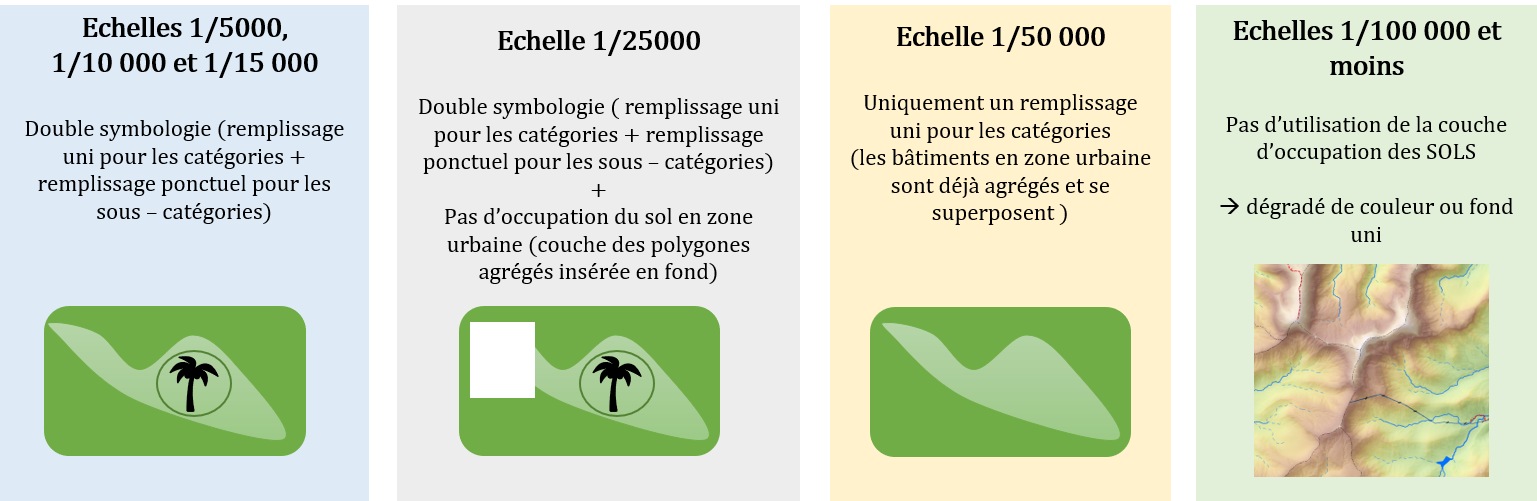
\includegraphics[width=\linewidth]{images/chap2/OCS.png}
\caption{Explication schématique de l'utilisation de la couche d'occupation des sols}
\label{ocs}
\end{figure}

\subsection{Cas des zones récifales lagonaires}

La cartographie des îles de la Polynésie est indissociable de la cartographie des récifs qui représentent des éléments incourtanables du relief. La section Topographie maintient dans sa base de donnée une couche d'entités linéaires
\textit{"HYD\_limite\_eau"}. Les multilignes tracent le contour des pâtés de coraux et des récifs mais cette couche est difficilement utilisables car imprécises. Par ailleurs, ce n'est pas une couche surfacique et elle ne permet pas, même avec des transformations sur SIG de distinguer les teintes de couleur des récifs.
Les cartes papier utilisent d'autres produits appelés fond cyan raster qui corespondent à des orthophotos rectifiée\footnote{la bande bleue est symbolisée par une échelle de cyan} et qui ont l'avantage de donner une représentation précise des zones littorales. Si les fonds cyans sont pertinents pour des échelles allant du 1/50 000 au 1/5000, ils ne le sont plus pour des échelles plus petites. La solution de contournement est l'utilisation de données de télédétection issues de ....
Un travail important permettant de simplifier les très nombreuses catégories scientifiques et les regrouper a été effectué. Il s'est notamment appuyé sur  l'Atlas des récifs coralliens de Polynésie française publié par des chercheurs néo-calédoniens en 2005 \cite{Noumea_2005}.
Elles permettent de classer les récifs de manière plus ou moins précises permettant de faire ressortir les zones d'eau peu profonde (couleur turquoise) ainsi que les barrières de corail. Ainsi, la cartographie au 1/500 000 ne fait figurer que les barrières de corail.

Cependant, ces dalles raster présente un désavantage majeur. Un masque turquoise ( couleur \#96DDFF ) à 100m des côtes doit être superposé aux dalles raster de forme carrée pour harmoniser les îles. Cependant, les teintes de bleu des dalles ne sont pas les mêmes d'îles en îles et posent donc un problème dès que la cartographie ne se limite plus à une seule île. Ce problème n'a pas été résolu et demeure donc sur les cartes dites "papier". En ce qui concerne l'export web, les limitations concernant l'usage de raster ont conduit à des choix de cartographie différents exposés dans le dernier chapitre.



\section {Placement des étiquettes}

Une des difficultés inhérentes au placement des étiquettes est la lisibilité. Les étiquettes doivent être adaptées à l'échelle et du 1/500 000 au 1/15 000, il n'existe pas dans la BD de la DAF de groupe d'annotations générées. Ainsi les étiquettes doivent être construites à partir des couches de points d'activités et des couches de toponymes. Le travail de généralisation n'est pas à faire. En effet pour ces deux couches, un champ \textit{"importance"} indique déjà les éléments à sélectionner. Le coeur du travail réside donc dans le placement et le style de celles-ci.

\begin{figure}[ht]
\centering
\includegraphics[width=\linewidth]{images/chap2/etiquette.jpg}
\caption{Carte de Papeete (généralisée pour l'échelle 1/25 000) permettant de visualiser les étiquettes}
\label{25eti}
\end{figure}

Si les couches \textit{NOM\_PAI} et \textit{NOM\_TOPONYME} représentent une grande partie des étiquettes sur les cartes, l'étiquetage se fait également sur des couches d'entités destinées à l'affichage comme les bornes kilométriques, les cours d'eau, ou encore les courbes de niveau.

\begin{center}
    Quelles contraintes respecter ?
\end{center}

La principale est bien entendu la cohérence des étiquettes entre les échelles. C'est une condition sine qua non au repérage de l'utilisateur entre les différentes échelles. Le code couleur doit donc être cohérent, ainsi que la police et sa taille. On observe sur la figure \ref{25eti} le travail réalisé à l'échelle 1/25 000. Plus de résultats peuvent être consultés en annexe.
On notera que la position des étiquettes par rapport à l'ombrage influe beaucoup sur le rendu final. Le choix qui a été effectué, influencé par la nécessité d'avoir une grande lisibilité, est de placer les étiquettes au dessus de l'ombrage à l'exception de celles concernant les courbes de niveau, car l'effet obtenu semble augmenter la perception du relief.

\begin{center}
    \textit{Quelques remarques sur les améliorations possibles et les problèmes d'étiquetage :}
\end{center}

En terme de symbologie, certains pictogrammes ont vocation à être améliorés comme pour les cascades. Un travail intéressant mais long et fastidieux serait de répertorier un angle d'orientation dans un champ de la table permettant d'orienter les symboles comme c'est le cas pour les noms des passes par exemple. Ensuite, les symboles des bornes kilométriques n'est pas satisfaisant. Une bonne représentation serait d'utiliser la forme des bornes réelles (se référer à la photo dans le glossaire), en plaçant l'étiquettes directement sur le symbole et au bon endroit. C'est un travail particulièrement long et technique nécessitant une très bonne maîtrises des outils d'étiquetage d'ArcGIS. Enfin, parmi les défauts d'étiquetage qui persistent après les multiples versions de cartes en papier, figure l'étiquetage des quartiers à Papeete. Il se fait par un texte noir entouré d'un halo blanc. Cependant, au milieu des nombreux bâtiments de la capitale, affichés en noir sur fond blanc à cette échelle, le résultat est mitigé. Il pourrait peut-être être amélioré par des traitements spécifiques à la capitale polynésienne ou par un changement dans la couleur des bâtiments qui serait alors problématique pour le rendu partout ailleurs.



\section {Résultats aux différentes échelles}

Pour valider le travail et savoir quelles corrections apporter, des échantillons de cartes ont été imprimés au format A0 pour un retour de l'ensemble des géomètres et géomaticiens de la section topographie de la DAF. Leurs remarques ont permis de retravailler certains algorithmes de généralisation ou encore certaines symbologies, police d'écriture ou couleur de fond de carte. 

La figure \ref{25_eti} ci-dessous présente un échantillon de  la carte au 1/25000 tandis que la figure \ref{100} est un extrait de la carte au 1/100 000. Compte-tenu du nombre d'échelles (8 niveaux) , l'ensemble des résultats figurent en annexe. Ces résultats ne sont pas ceux qui seront affichés sur le web. En effet, la publication des données dans un portail web nécessite de nombreuses simplifications qui font l'objet de la partie suivante. Par ailleurs, le portail web tient compte d'éventuelles retouchent liées au support de lecture et à l'harmonisation entre les niveaux de zoom. 
Cependant, ces supports papiers étaient indispensables à la préparation des couches en vue de l'export web. Ils pourront aussi servir après d'éventuelles retouches à fournir des exemplaires papiers sur demande des clients.

\begin{figure}[!h]
\centering
\includegraphics[width=5cm]{images/chap2/etiquette.jpg}
\caption{Carte centrée sur le nord de Tahiti (généralisée pour l'échelle 1/100 000)}
\label{100}
\end{figure}

\section{Remarques et critiques sur les choix de cartographie}
{\color{magenta} NON REDIGE : Liste des choses qui ne vont toujours pas sur les cartes, excepté les problèmes d'étiquetage évoqués plus haut}
